\documentclass[UTF8,a4paper,landscape,10pt,fontset=fandol]{ctexart}
\usepackage[margin=16mm,headheight=14pt]{geometry}
\usepackage{amsmath,amssymb,booktabs,tabularx,array,graphicx,xcolor,hyperref,fancyhdr,multicol}
\definecolor{ink}{HTML}{174D78}
\hypersetup{colorlinks=true,urlcolor=ink,linkcolor=ink,pdftitle={氘核：实验与Fortran计算比较},pdfauthor={含时量子多体调研项目}}
\setlength{\emergencystretch}{2em}\setlength{\parindent}{0pt}\setlength{\parskip}{4pt}
\setlength{\tabcolsep}{5pt}\renewcommand{\arraystretch}{1.4}
\pagestyle{fancy}\fancyhf{}\fancyhead[L]{氘核：实验与Fortran计算比较}\fancyhead[R]{EM500\quad 2026-09-29}\fancyfoot[C]{\thepage}
\newcommand{\pct}{\%}
\begin{document}
{\LARGE\bfseries\color{ink} 氘核观测量：计算与实验比较}\par
核力采用现有固定EM500；结合能和波函数由Fortran直接求解。本次增加坐标波函数、半径、密度、冲量近似电磁矩及渐近量输出；\textbf{未重新拟合核力，也未用实验值修正计算结果}。

\begin{tabularx}{\textwidth}{@{}p{63mm}p{33mm}p{53mm}p{31mm}X@{}}
\toprule
观测量 & 本次计算 & 实验/评价或提取值 & 偏差 & 备注 \\
\midrule
结合能 $B_d$（MeV） & 2.22457528 & $2.2245662(4)$ [1] & $+9.08$ eV & 历史定参 \\
电荷半径 $r_{\rm ch}$（fm） & $\approx 2.12677$ & $2.12778(27)$ [2] & $-0.00101$ fm & 近似估计 \\
电四极矩 $Q_d/e$（fm$^2$） & 0.274951 & $0.285699(15)(18)$ [3] & $-3.76\pct$ & 冲量近似 \\
磁矩 $\mu_d$（$\mu_N$） & 0.854087 & $0.8574382335(22)$ [2] & $-0.391\pct$ & 冲量近似 \\
S波渐近系数 $A_S$（fm$^{-1/2}$） & 0.88430 & $0.8845(8)$ [4] & $-0.022\pct$ & np分析提取 \\
渐近D/S比 $\eta$（无量纲） & 0.02558 & $0.0256(4)$ [5] & $-0.075\pct$ & 反应分析提取 \\
\bottomrule
\end{tabularx}

\textbf{半径能否对上？} 近似电荷半径与实验相差约 0.0010 fm，量级很接近，但尚未完全落入表列实验误差范围。此处遗漏电磁算符修正，且输入核子半径有误差和相关性，不能把该差值直接判为核力误差，或当作完整精度验证。

\textbf{表中记号。} 百分数为 $(\text{计算}/\text{实验}-1)\times100\%$，不是误差显著性。括号为末位不确定度；四极矩的两组括号分别来自分子理论和实验提取。计算列保留的数字不代表模型达到同等物理精度。

\textbf{结合能说明。} 结合能是EM500的历史定参量，不是独立预测。固定力的历史目标为 $2.224575$ MeV；本次求得 2.22457528 MeV。与现代AME2020的约9 eV差异应区别于求解网格误差，不在本轮重新调整参数。

\textbf{电磁量说明。} 电荷半径估计仅计入核子有限尺寸与Darwin--Foldy项；四极矩、磁矩采用单核子冲量近似（IA）。双核子电荷、双核子电流及其他电磁修正尚未完整计入。

\textbf{渐近量说明。} 表列 $A_S$ 的经验值来自低能np散射分析，$\eta$ 的经验值来自反应分析，均非直接密度测量。$\eta$ 是渐近振幅比，与D态概率不同。

\textbf{其他波函数量。} 点核子半径 $r_{\rm pt}=1.97450$ fm，采用 $R=r/2$ 约定，不能直接与实验电荷半径比较；n--p均方根间距为 3.94899 fm；D态概率为 4.5142\%。D态概率依赖相互作用及表示，没有直接实验对照。
\newpage
{\Large\bfseries\color{ink} 密度分布与半径的关系}\par
$r$表示两个核子之间的距离，$R=r/2$表示核子到等质量几何中心的距离。波函数归一为 $\int_0^\infty [u^2(r)+w^2(r)]\,dr=1$。下图是未极化氘核的球平均\textbf{点核子}分布，并非实验电荷密度。
\[
P(r)=u^2(r)+w^2(r),\qquad
\rho_N(R)=\frac{u^2(2R)+w^2(2R)}{\pi R^2},\qquad
\int 4\pi R^2\rho_N(R)\,dR=2,\qquad
r_{\rm pt}^2=\frac14\int r^2P(r)\,dr.
\]
\begin{center}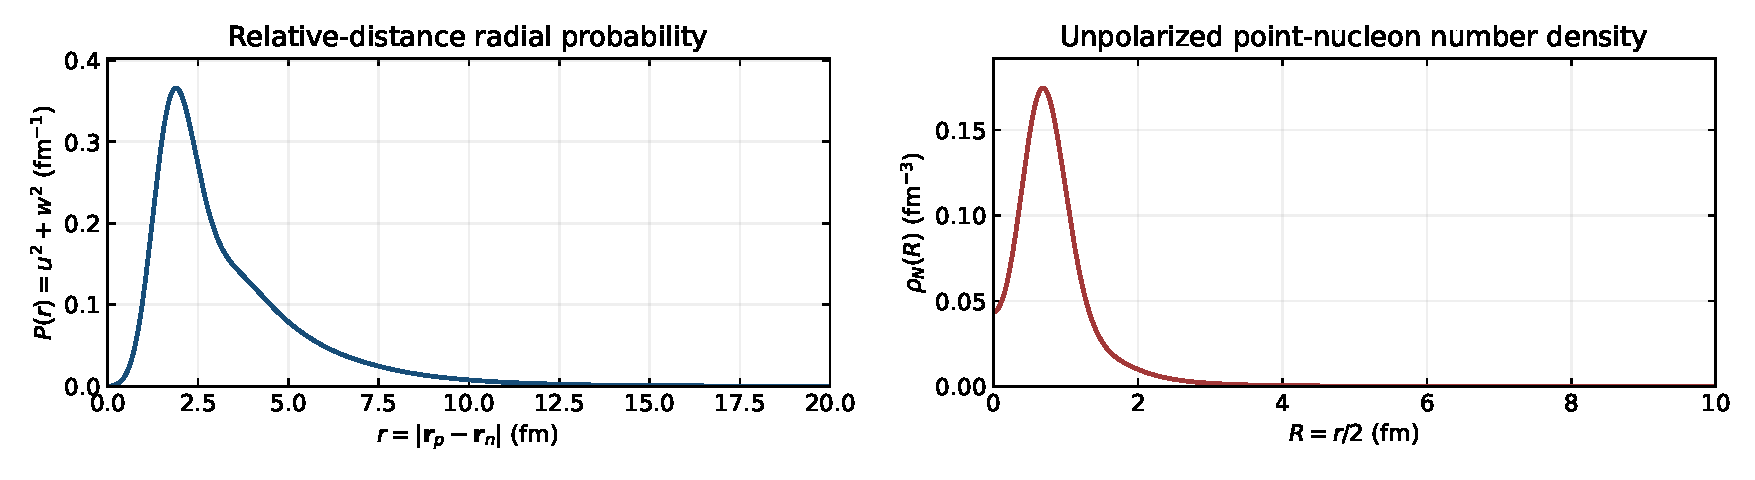
\includegraphics[width=0.97\textwidth]{deuteron_density.pdf}\end{center}
电荷半径估计采用一致的标准约定 [6]：
\[
r_{\rm ch,est}^{\,2}=r_{\rm pt}^{\,2}+r_p^2+\langle r_n^2\rangle+\frac34\left(\frac{\hbar c}{m_pc^2}\right)^2,
\quad r_p=0.84075\ {\rm fm},\quad \langle r_n^2\rangle=-0.1155\ {\rm fm}^2.
\]
其中Darwin--Foldy项约为0.03317 fm$^2$；额外自旋轨道和双核子电荷算符等未计入。中子均方电荷半径为负不表示物质半径为负。

\textbf{密度能和什么实验比较？} 电子散射测量的是形状因子或相关观测量，例如 $G_C,G_Q,G_M$（通过 $A,B,T_{20}$ 等提取）。它们提供电荷与磁分布信息，但从本图的点核子密度到这些实验量还需核子形状因子和电磁算符；本轮未计算这些有限动量转移量，未列逐点实验密度。

\textbf{程序状态。} 原程序已有结合能和动量波函数输出；本次已补齐以上坐标分布、半径、IA电磁矩和渐近量的Fortran计算。完整电荷/磁形状因子及一致的双核子电磁算符仍未实现。对自旋定向氘核，密度还可具有角度依赖，本图只展示未极化球平均。
\newpage
{\Large\bfseries\color{ink} 数值设置、复现与来源}\par
\textbf{本次设置：} 动量Gauss网格192点，积分上限1000 MeV/$c$；相对坐标 $0\le r\le60$ fm，步长0.01 fm；渐近量在20--25 fm窗口拟合，衰减常数 $\gamma=\sqrt{mB_d}/(\hbar c)$ 固定，$m=2M_pM_n/(M_p+M_n)$，质量以能量单位计。坐标波函数未再次人为归一化，坐标与动量归一化差为 $-1.44\times10^{-12}$。

\textbf{输出与复现：} 本目录保存输入、实际Fortran运行结果、实验来源、CSV比较表、密度图和本PDF的源文件。运行 \texttt{./run\_deuteron.sh} 重新计算；\allowbreak 运行 \texttt{python3 build\_report.py} 重建表与图（需Matplotlib和XeLaTeX）。主程序新增 \texttt{write\_coordinate=.true.}；统一代码根目录中的 \texttt{input\_deuteron\_observables.nml} 是可用示例。计算仍由Fortran完成，Python只读结果并排版。

\textbf{来源与数据性质：}
\begin{enumerate}
\item AME2020官方质量表，$^2$H的结合能/核子为1112.2831(2) keV，乘2得到表列值。\href{https://www-nds.iaea.org/amdc/ame2020/mass_1.mas20.txt}{IAEA原始表}。
\item CODATA 2022（2025年发布）：氘核电荷半径、磁矩、质子半径及核子磁矩。\href{https://physics.nist.gov/cuu/Constants/Table/allascii.txt}{NIST官方数表}。中子均方电荷半径采用\href{https://pdg.lbl.gov/2025/listings/rpp2025-list-n.pdf}{PDG 2025}的 $-0.1155(17)$ fm$^2$；这些是附加电磁输入，未替换原核力质量或参数。
\item Puchalski, Komasa, Pachucki, Phys. Rev. Lett. \textbf{125}, 253001 (2020)：四极矩来自分子精密测量与理论分析。\href{https://doi.org/10.1103/PhysRevLett.125.253001}{原论文}，\href{https://arxiv.org/pdf/2010.06888}{公开全文}。
\item de Swart, Terheggen, Stoks, \emph{The Low-Energy np Scattering Parameters and the Deuteron} (1995)，低能np分析提取的 $A_S=0.8845(8)$。\href{https://arxiv.org/pdf/nucl-th/9509032}{原文}。
\item Rodning and Knutson, Phys. Rev. C \textbf{41}, 898 (1990)，亚库仑转移反应提取 $\eta=0.0256(4)$。\href{https://doi.org/10.1103/PhysRevC.41.898}{原论文}。
\item Filin等，Phys. Rev. C \textbf{103}, 024313 (2021)，式49--52及附录A：点核子半径、结构半径、电荷半径及电磁算符的区别。\href{https://arxiv.org/pdf/2009.08911}{公开全文}。
\item Machleidt与Entem，Phys. Rep. \textbf{503}, 1--75 (2011)，表9给EM500的舍入理论基准：$r_{\rm pt}\simeq1.975$ fm、$Q_{\rm IA}\simeq0.275$ fm$^2$、$A_S\simeq0.8843$、$\eta\simeq0.0256$、$P_D\simeq4.51\%$；这些是理论基准，不是实验值。\href{https://arxiv.org/pdf/1105.2919}{公开全文}。
\end{enumerate}
\textbf{结论边界：} 波函数给出的点核子半径约为1.9745 fm；加入有限核子尺寸等后，电荷半径估计约为2.1268 fm，与实验接近。四极矩和磁矩存在可见IA偏差，完善比较需要一致的电磁算符。数值收敛与物理模型精度应分开判断。
\end{document}
